\section{Виртуальный эксперимент}

Для обучения и тестирования CLaNN мы использовали синтетические  данные двухосного растяжения и раздувания гиперупругой мембраны соответственно.
% Мы используем синтетические экспериментальные данные для тестирования CLaNN 
% на изотропном надуваним однородной и неоднородной по толщине мембраны. 
% А именно, мы генерируем данные с помощью виртуальных экспериментов на плоских растяжениях образца и используем их в качестве входных данных для 
% обучения CLaNN, без какого-либо дополнительного знания об изотропности/анизотропности образца и форме потенциала.
Обучение модели проводилось на численных экспериментальных данных, 
полученных при двухосном растяжении образца с геометрией "мальтийский крест" и толщиной $H=0.53$ мм (Рисунок \ref{fig:malt_geometry}) методом гиперупругой узловой силы \cite{ddaniso2024}. 
Материал мембраны задавался неогуковской моделью \cite{ogden1997nonlinear}:
\begin{align} \label{eq:neohook}
        \widetilde{\psi} &= \dfrac{\mu H(X)}{2} (I_1 +J^{-2}-3),
        \quad     I_1 = e^{2\xi_1} (1+\xi_3^2)+e^{2\xi_2},\quad J = e^{\xi_1+\xi_2}
\end{align}
с $\mu=0.43\cdot 10^6$ Па.

% Данные для обучения извлекались из различных областей образца...

% Для решения задачи равновесия гиперупругой мембраны используется метод описанный в \cite{ddaniso2024}.

\begin{figure}[H]
  \centering
  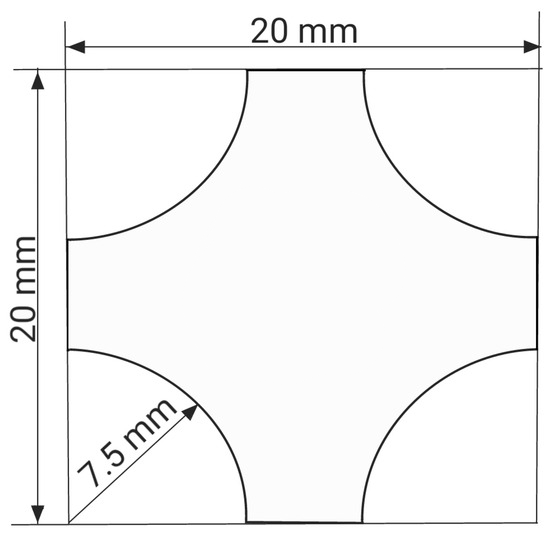
\includegraphics[width=0.4\textwidth]{img/malt_geom.png}
  \caption{Размеры образца биоматериала в форме мальтийского креста. 
  Радиус вырезов одинаков для всех вырезов}
  \label{fig:malt_geometry}
  \label{fig:malt_displacements}
\end{figure}

Схема нагружения образца показана на рисунке \ref{fig:malt_displacements}, где $w_i \in [0,1]$, $i \in \{1,4\}$
представляет собой долю от заданного максимального смещения $u_{\max}$ для $i$-го плеча: $w_i = 0$ 
соответствует неподвижному плечу, а $w_i = 1$ — соответствует плечу, чьё положение было сдвинуто и фиксировано на расстояние $u_{max}$. 
Изменяя $w_i$, можно получить различные варианты двухосного нагружения. 
В наших виртуальных экспериментах мы последовательно
смещаем плечи с приращением $\Delta s$. 
Смещение $w_i \cdot n \cdot \Delta s$ прикладывается к $i$-му плечу на $n$-м шаге, где $n = 1, \ldots, N$, 
$N = u_{\max}/\Delta s$ — количество шагов. 
Метод гиперупругой узловой силы применялся к изначально плоской квазиоднородной неструктурированной триангуляции с шагом сетки $h=0.5$ мм и размером $5 404$ треугольников. Максимальное смещение плеча
$u_{\max} = 2$ мм и $\Delta s = 0.2$ мм.
На каждом шаге извлекались $\mathbb{C}, \mathbb{S}$ для всех треугольников, принадлежащих выбранной области наблюдения. 
% Поскольку мы используем линейные ($P_1$) конечные элементы, значения $(\vect C, \vect S)$ постоянны на каждом треугольнике.

 
 
Наш предлагаемый тестовый протокол предполагает девять экспериментов:

\begin{figure}[H]
  \centering
  \begin{minipage}[t]{0.48\textwidth}
    \centering
    \vspace{0pt}
    \begin{tabular}{|c|c|c|c|c|}
    \hline
    \textbf{№} & $w_1$ & $w_2$ & $w_3$ & $w_4$ \\
    \hline
    1 & 1 & 1 & 1 & 1 \\
    2 & 1 & 0.75 & 1 & 0.75 \\
    3 & 0.75 & 1 & 0.75 & 1 \\
    4 & 1 & 0.5 & 1 & 0.5 \\
    5 & 0.5 & 1 & 0.5 & 1 \\
    6 & 1 & 1/3 & 1 & 1/3 \\
    7 & 1/3 & 1 & 1/3 & 1 \\
    8 & 1 & 0 & 1& 0 \\
    9 & 0 & 1 & 0 & 1 \\
    \hline
    \end{tabular}
    \captionof{table}{Протоколы тестовых экспериментов}
    \label{tab:test_protocols}
  \end{minipage}\hfill
  \begin{minipage}[t]{0.48\textwidth}
    \centering
    \vspace{0pt}
    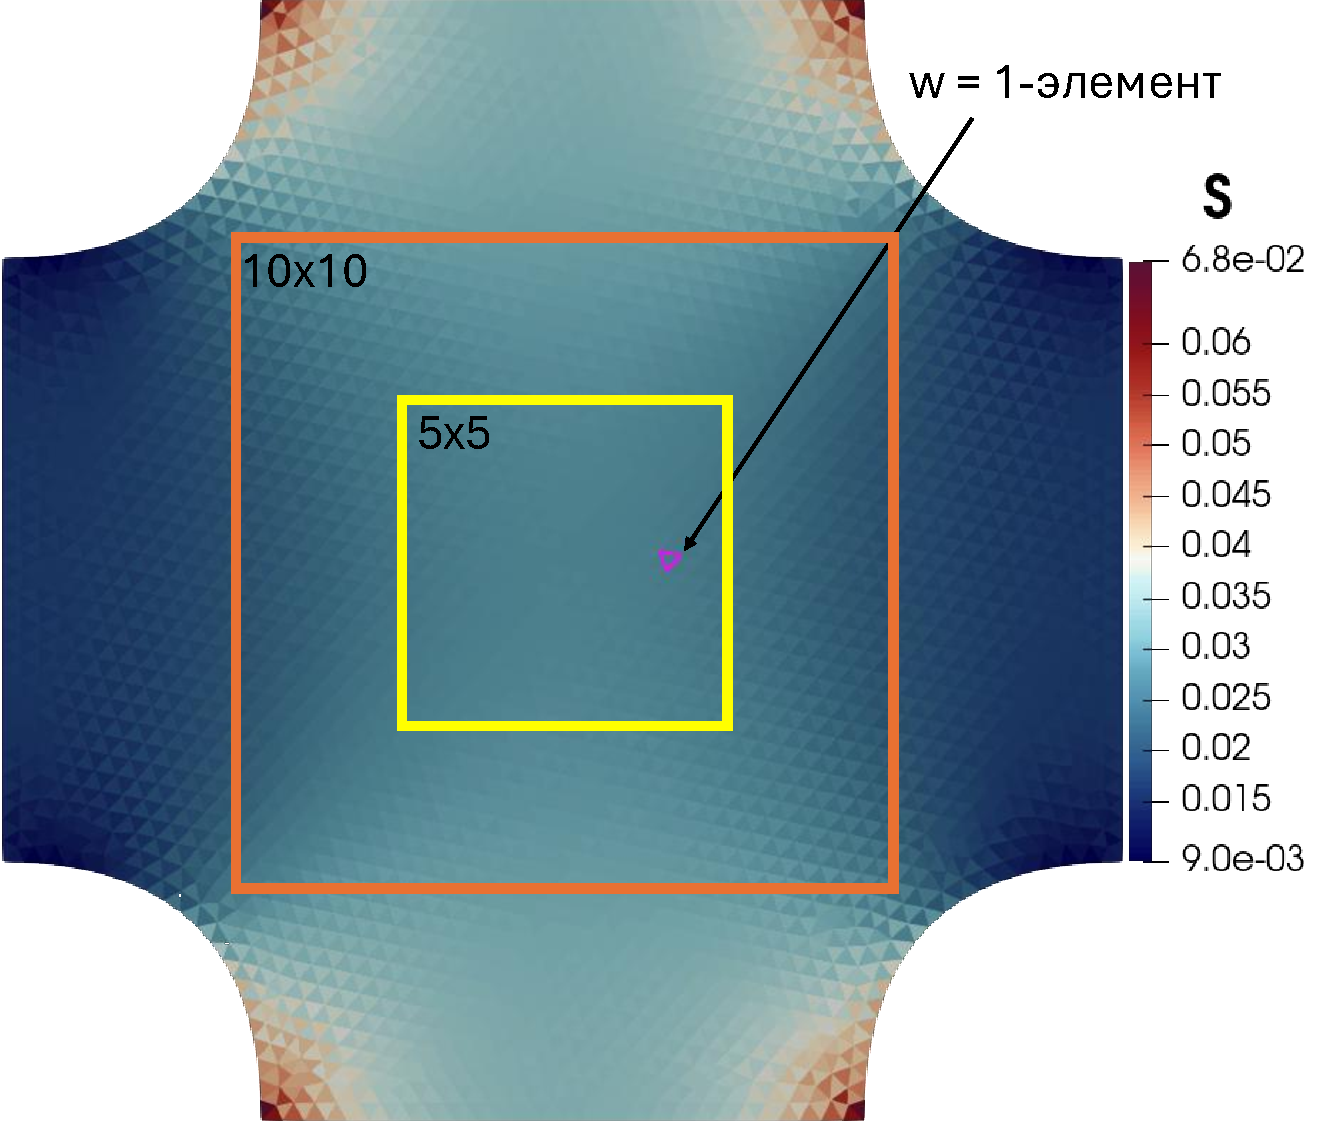
\includegraphics[width=\linewidth]{img/Numerical/malt_window.pdf}
    \captionof{figure}{Поле напряжения $\vect S$ деформированной мембраны с геометрией "мальтийский крест" с различными окнами наблюдения $w$.}
    \label{fig:malt_window}
  \end{minipage}
\end{figure}

\subsubsection{Правила отбора данных}
\paragraph{Центральное окно $w$.}
Окно задаётся в исходной конфигурации $\Omega_0$ как центральная область вокруг геометрического центра 
образца, согласованная с осями расчётной сетки.
Для $w=5\times5$ мм и $w=10\times10$ мм берётся квадрат со сторонами 5 и 10 мм соответственно, 
центрированный в центре образца; для $w=\text{всё поле}$ — вся область $\Omega_0$.
Для $w=\text{1-элемент}$ берётся единственный центральный треугольник 
(ячейка с минимальным номером на вычислительной сетке для окна 5x5 мм $\Omega_0$ как показано на рисунке \ref{fig:malt_window} ).
Наблюдения включают все треугольники, барицентры которых $\mathbf{X}_T$ лежат внутри выбранного окна $\mathcal{W}_w\subset\Omega_0$.
% TODO: добавить мощность окна в элементах сетки

\paragraph{Состав наблюдений (данные).}
На каждом шаге нагружения $n=1,\dots,N$ и для каждого треугольника $T\in\mathcal{T}_w$ (ячейки, попавшие в окно) фиксируется пара $(\vect C_T^{(n)},\,\vect S_T^{(n)})$, 
где $\vect C$ — правый тензор Коши–Грина, $\vect S$ — второй тензор Пиолы–Кирхгофа.
Единицы: размеры окна — мм; $\vect C$ — безразмерен; $\vect S$ — МПа. 
При этом количество элементов сетки в окне наблюдения $|\mathcal{T}_w|$ для различных окон различно: 
$1$ для $w=\text{1-элемент}$, $252$ для $w=5\times5$ мм, $954$ для $w=10\times10$ мм и $5404$ для $w=\text{всё поле}$.

\paragraph{Формирование выборок.}
Для фиксированных $(p,w)$ совокупность всех пар $(\vect C_T^{(n)},\,\vect S_T^{(n)})$ образует базовый набор $D(p,w)$, из которого формируются разбиения $D_{\mathrm{tr}}(p,w)$ и $D_{\mathrm{val}}(p,w)$.
Для заданных протокола $p$ (см. табл.~\ref{tab:test_protocols}) 
и окна центральной области образца 
$w\in\{\text{1-элемент},\,5\times5\,\text{мм},\,10\times10\,\text{мм},\,\text{всё поле}\}$ обозначим
\[
  D_{\mathrm{tr}}\equiv D_{\mathrm{tr}}(p,w),\qquad D_{\mathrm{val}}\equiv D_{\mathrm{val}}(p,w),
\]
где $D_{\mathrm{tr}}$ — обучающая, $D_{\mathrm{val}}$ — валидационная выборки.



Например, |D(\{1..10\}, \text{1-элемент})|= 90 точек данных правого тензора деформаций Коши-Грина $\vect C$ 
и второго тензора напряжений Пиолы-Кирхгофа $\vect S$ (Рисунок \ref{fig:training_data}).

\begin{figure}[H]
  \centering
  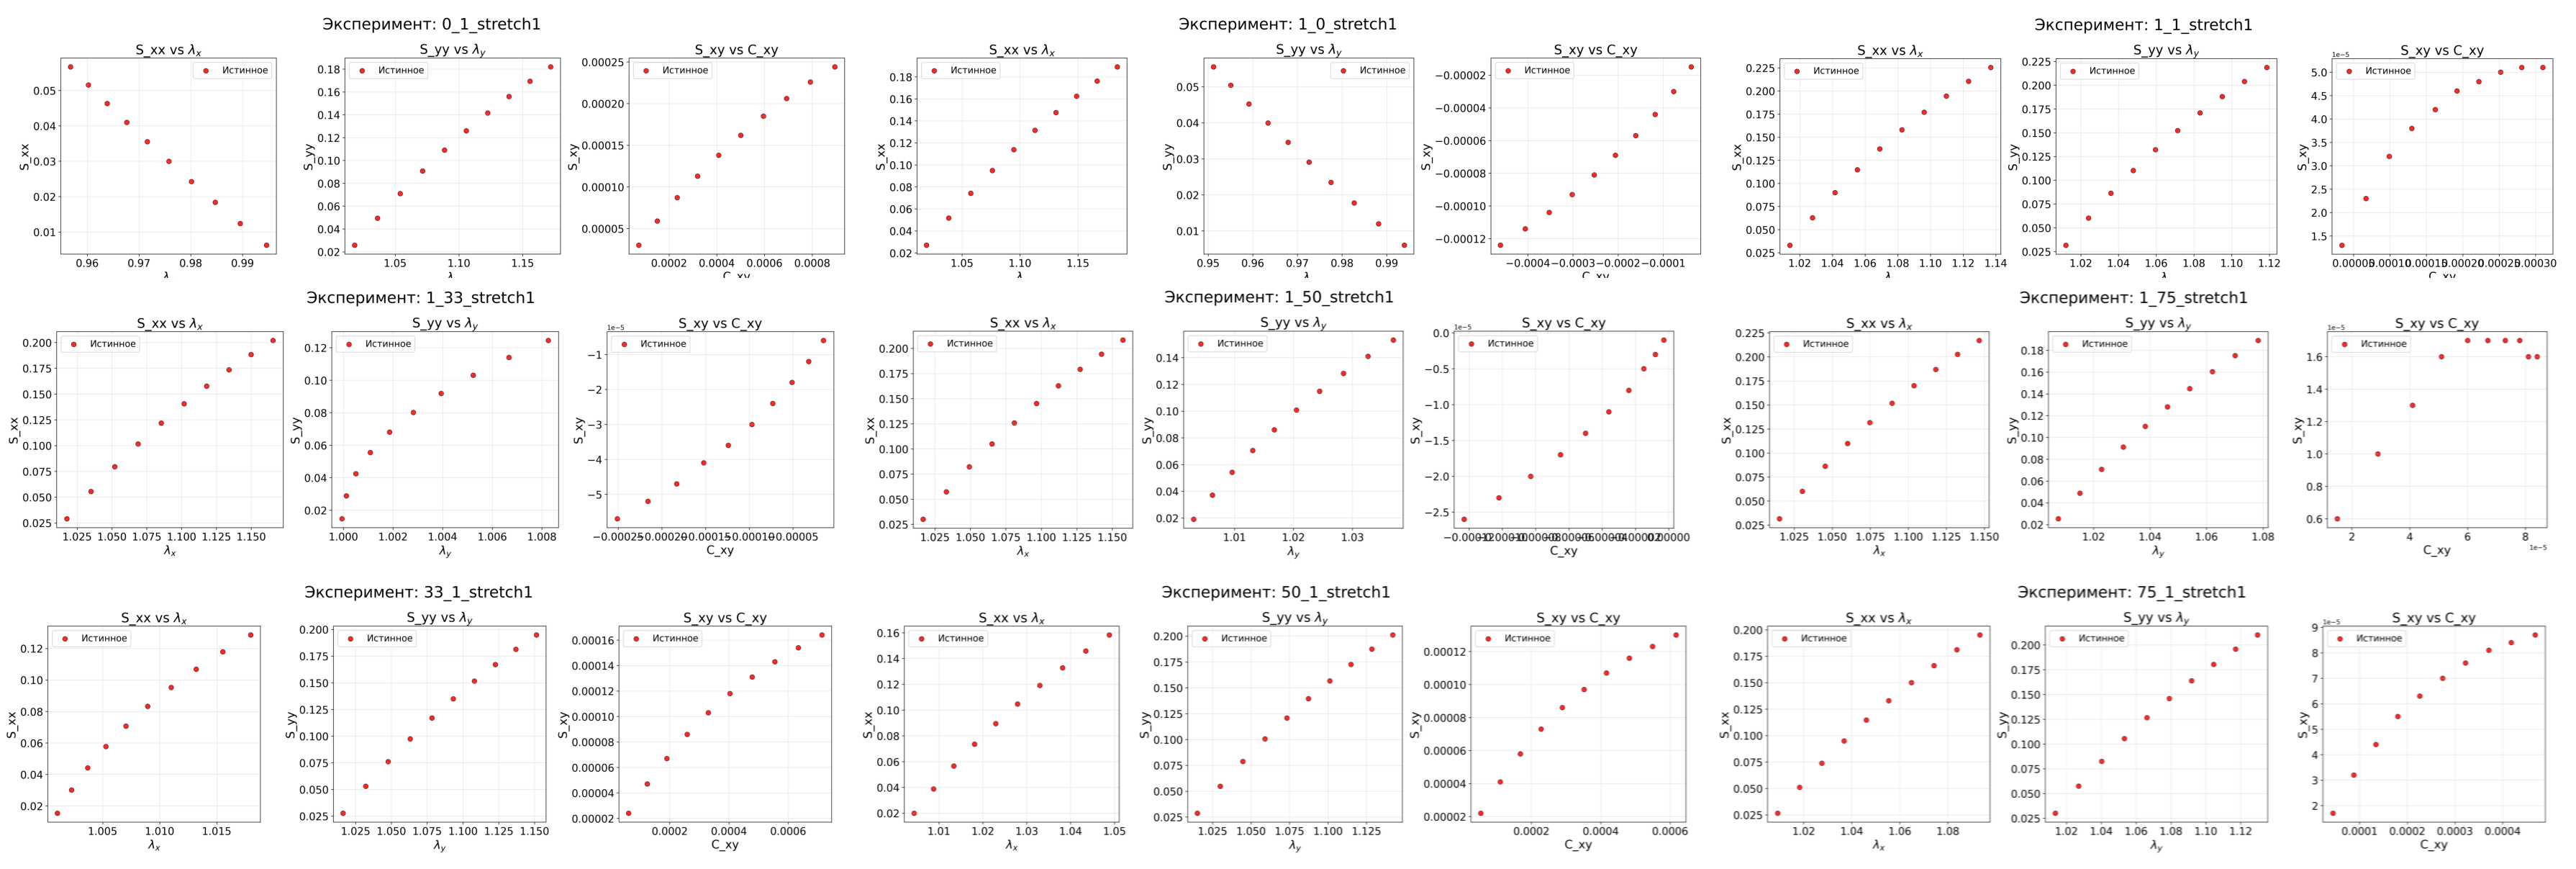
\includegraphics[width=1.0\textwidth]{img/all_stress_plots.png}
  \caption{Обучающий набор данных}
  \label{fig:training_data}
\end{figure}

Так как мы собираем данные из одного центрального элемента сетки, то растягивающие компоненты $xx, yy$ тензоров деформации $\vect C$ и напряжения
$\vect S$ имеют значения на 2-3 порядка большие чем сдвиговые компоненты $xy$.

\subsubsection{Метрики и критерии качества}
\label{sec:metrics}

Для количественной оценки качества предсказаний используем интегральные и точечные метрики, согласующиеся с энергетической нормой из вариационной постановки задач упругости (см., например, \cite{ciarlet1988mathematical,ogden1997nonlinear,holzapfel2000nonlinear}).

\textbf{Коэффициент детерминации $R^2$.}
\begin{equation}\label{eq:r_squared}
  R^2 = 1 - \frac{\sum_{i=1}^n (y_i - \hat{y}_i)^2}{\sum_{i=1}^n (y_i - \bar{y})^2},
\end{equation}
где $y_i$ — экспериментальные значения, $\hat{y}_i$ — предсказания модели, $\bar{y}$ — среднее экспериментальных значений, $n$ — число точек. Назначение: удобно сравнивать кривые нагружения; даёт нормированную меру согласия по траекториям.

\textbf{Точечная относительная ошибка.}
\begin{equation}\label{eq:rel_error}
  \epsilon = \frac{\| \vect S - \vect S_{\text{ref}} \|}{\| \vect S_{\text{ref}} \|}.
\end{equation}
% Назначение: отрисовка поля ошибки и его локальной структуры; наглядна на картах.

\textbf{P1-ошибка} \cite{xie2024p1} — комбинация абсолютной и относительной ошибок, чувствительная к малым значениям:
\begin{equation}\label{eq:p1_error}
  \epsilon_{\mathrm{P1}} = \frac{\| \vect S - \vect S_{\text{ref}} \|}{s_0 + \| \vect S_{\text{ref}} \|},\qquad s_0 = \max(\vect S_{\text{pred}}).
\end{equation}

\textbf{Абсолютная интегральная ошибка (L2 по сетке) для напряжений (Фробениус-норма).}
\begin{equation}\label{eq:l2_abs_stress}
  \|e\|_{L^2} = \Bigg( \sum_{K} \overline{\| \vect S_{\text{ref}} - \vect S_{\text{pred}} \|_F^{2}}^{\,K}\, |K| \Bigg)^{\tfrac12},
\end{equation}
где $|K|$ — мера ячейки (объём/площадь/длина). Для ячеечных данных усреднение по ячейке не требуется:
\begin{equation}\label{eq:l2_abs_stress_cell}
  \|e\|_{L^2} = \Bigg( \sum_{K} \| \vect S_{\text{ref},K} - \vect S_{\text{pred},K} \|_F^{2}\, |K| \Bigg)^{\tfrac12}.
\end{equation}
Назначение: сворачивает поле ошибки в скаляр и инвариантна к измельчению сетки (при фиксированном поле) \cite{BrennerScott2008,AinsworthOden2000,Verfurth2013}.

\textbf{Относительная интегральная ошибка.}
\begin{equation}\label{eq:l2_rel_stress}
  \|e\|_{L^2,\,\mathrm{rel}}\;=\; \frac{\Big( \sum\limits_{K} 
  \| \vect S_{\mathrm{ref},K} - \vect S_{\mathrm{pred},K} \|_F^{2}\, |K| \Big)^{\tfrac12}}
  {\Big( \sum\limits_{K} \| \vect S_{\mathrm{ref},K} \|_F^{2}\, |K| \Big)^{\tfrac12}}\,.
\end{equation}
% Назначение: корректное сопоставление сценариев с разными уровнями напряжений; нормировка на «энергетическую мощность» эталонного поля.


\textbf{Гиперпараметры оптимизации:}
\begin{itemize}
  \item Скорость обучения (learning rate): $0.001$
  \item Размер батча (batch size): $4$ при обучении на 90 точек данных и $128$ для остальных обучающих наборов данных.
  % \item Веса физических ограничений: $\lambda_{\text{SI}} = 0.1$, $\lambda_{\psi} = 0.1$
  \item Архитектура: 16 нейронов на скрытом слое
  \item Сглаживающий параметр $\beta$: $10$
\end{itemize}

\textbf{Результаты обучения:}
Процесс оптимизации показал высокую эффективность: ошибка аппроксимации снизилась на 5 порядков за менее чем 5000 эпох (рисунок \ref{fig:loss_curve}), 
что демонстрирует как качество предложенной архитектуры, так и корректность выбора гиперпараметров. 
Столь быстрая сходимость обусловлена строгой выпуклостью функции энергии, что обеспечивает единственность 
минимума и отсутствие локальных минимумов в пространстве параметров.

\begin{figure}[H]
  \centering
  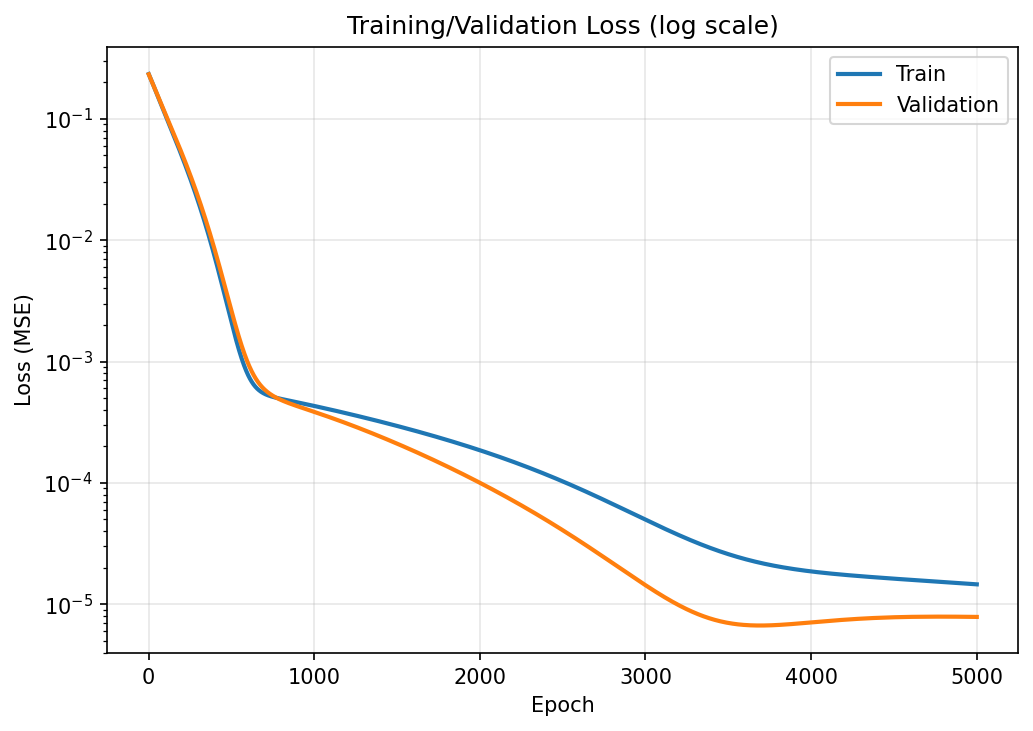
\includegraphics[width=0.7\textwidth]{img/loss_curve.png}
  \caption{Кривая функции потерь при обучении на 90 точках данных}
  \label{fig:loss_curve}
\end{figure}


\subsection{Интерполяция и экстраполяция кривых нагружения}
  Сначала мы проверили, как модель CLaNN интерполирует и экстраполирует кривые нагружения, используя выборки
  $D_{\mathrm{tr}}(p,w)$ и $D_{\mathrm{val}}(p,w)$ для заданного окна наблюдения $w$.
  Для оценки качества использовали коэффициент детерминации $R^2$ (см. раздел \ref{sec:metrics}, формулу \eqref{eq:r_squared}). Метрику качества фиксируем как:
\[
  R^2_{\alpha}(D_{\mathrm{val}}),\qquad \alpha\in\{xx,yy,xy\}.
\]

  \textbf{Интерполяция.}  

  Для тестирования способности архитектуры CLaNN к интерполяции кривых нагружения мы использовали данные из 
  10 точек кривой нагружения равнодвухосного растяжения мембраны $p=1$, 
  окно наблюдения $w=\text{1-элемент}$:
  
  $D_{in} = D(p{=}1,\,w{=}\text{1-элемент}),\, n = 1..10,$
  
  $D_{\mathrm{tr}}=\{\forall (\vect {C}^{n_{tr}}, \vect{S}^{n_{tr}}) \in D_{in}|\; n_{tr}=\{1,5,10\}\},$
  
  $D_{\mathrm{val}}=\{\forall (\vect {C}^{n_{val}}, \vect{S}^{n_{val}}) \in D_{in}|\; n_{val}=n \\  n_{tr}\}.$

  CLaNN показал высокую точность интерполяции кривой нагружения равнодвухосного растяжения мембраны 
  для растягивающих компонент $R^2_{xx}=0.999$, $R^2_{yy}=0.999$, и отсуствие достоверного предсказания сдвиговых 
  компонент $R^2_{xy}=0$ (рисунок \ref{fig:interpolation}).
  
  \begin{figure}[H]
    \centering
    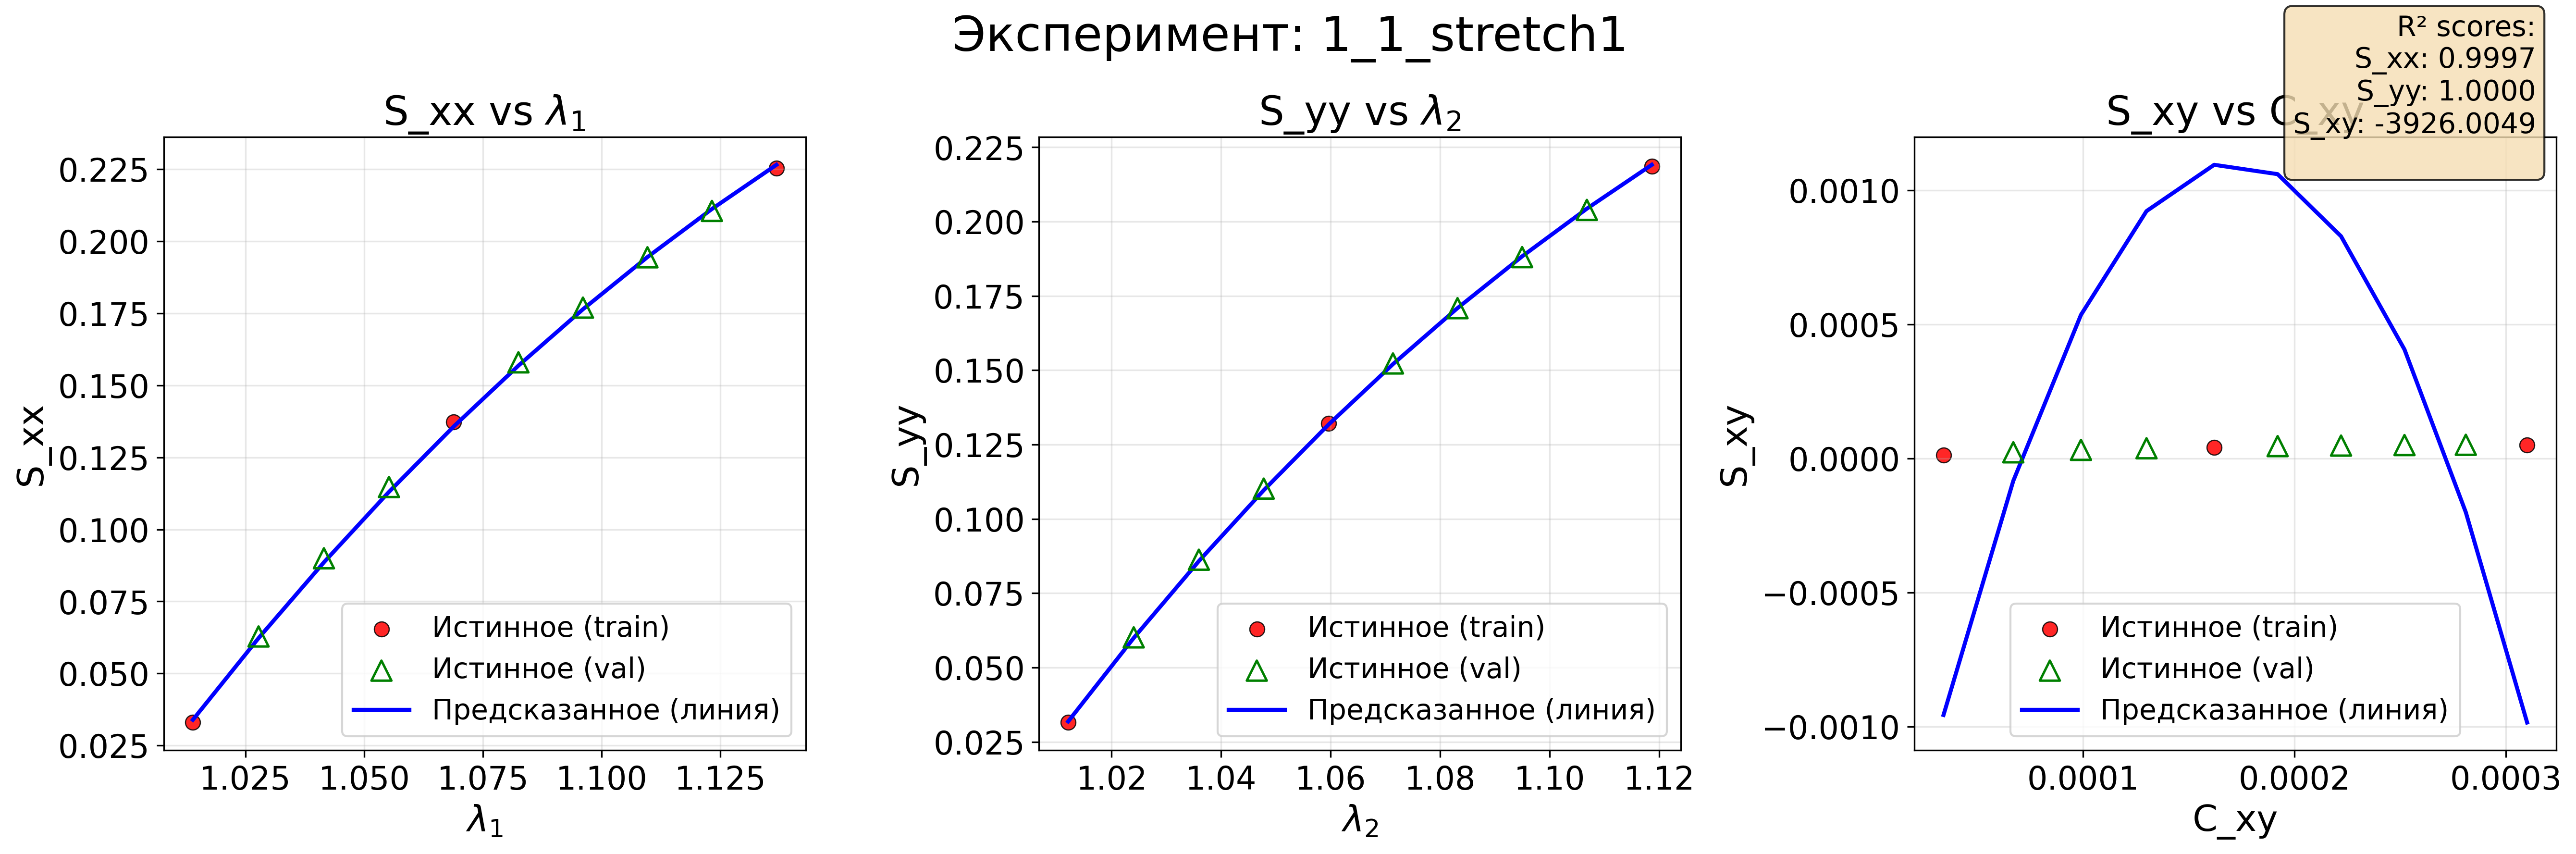
\includegraphics[width=1.0\textwidth]{img/interpolation.png}
    \caption{Кривая нагружения для равнодвухосного растяжения}
    \label{fig:interpolation}
  \end{figure}
  
  \textbf{Экстраполяция.}
  
  Для проверки способности CLaNN к экстраполяции кривых нагружения использовали обучение на равнодвухосном растяжении (p = 1) и валидацию на неравнодвухосном (p = 9), 
  окно наблюдения $w=\text{1-элемент}$:
  
  $D_{\mathrm{tr}} = D(p{=}1,\,w{=}\text{1-элемент}),\, n = 1..10,$
  
  $D_{\mathrm{val}} = D(p{=}9,\,w{=}\text{1-элемент}),\, n = 1..10,$
  
  CLaNN показал высокую точность экстраполяции для растягивающих компонент $R^2_{xx}=0.993$, $R^2_{yy}=1.0$, и отсутствие достоверного предсказания сдвиговой компоненты $R^2_{xy}=0$ (рисунок \ref{fig:extrapolation}).


  \begin{figure}[H]
    \centering
    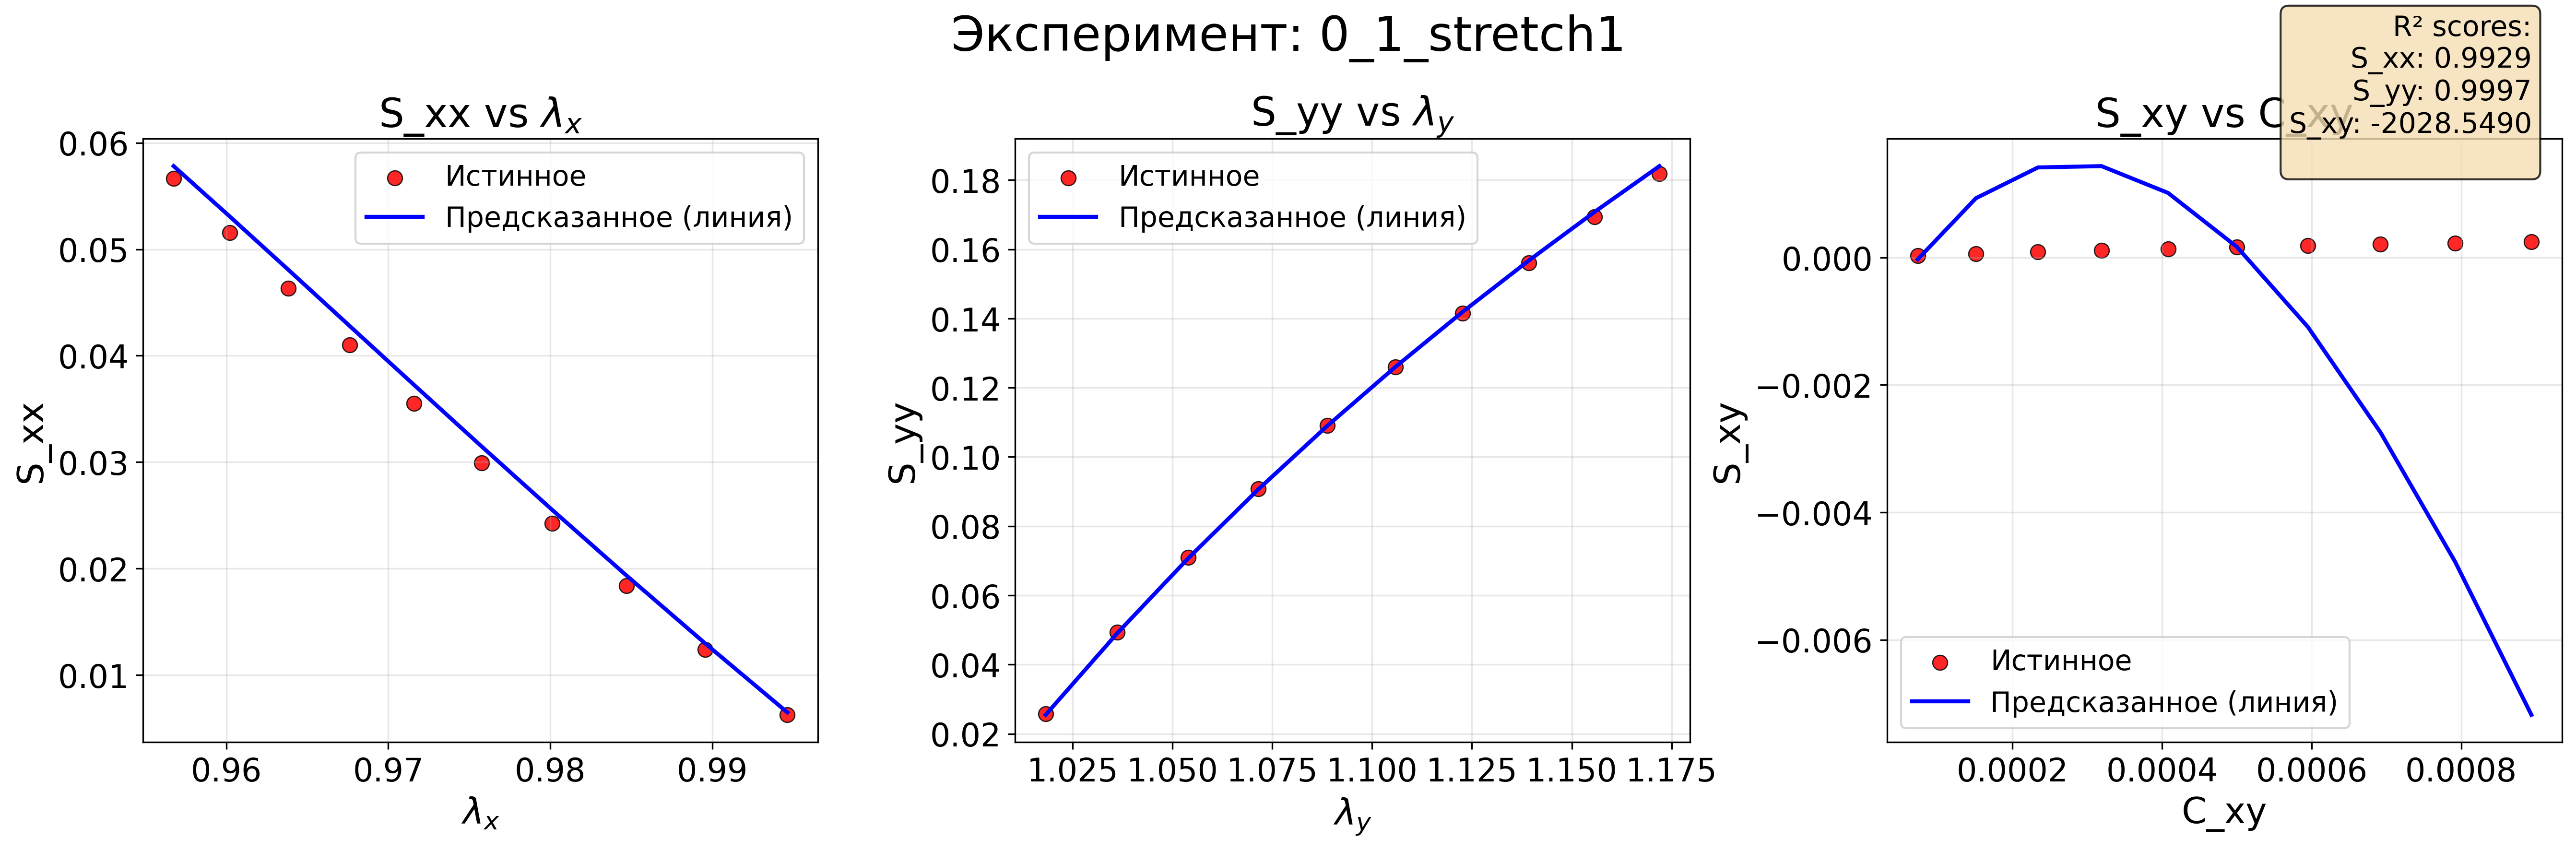
\includegraphics[width=1.0\textwidth]{img/extrapolation.png}
    \caption{Кривая нагружения для неравнодвухосного растяжения}
    \label{fig:extrapolation}
  \end{figure}
   
  Таким образом, CLaNN способен интерполировать и экстраполировать кривые нагружения с высокой точностью, что свидетельствует о его способности к обобщению на новые данные.
  Однако, не справляется с предсказанием сдвиговых компонент $\vect S_{xy}$, что может быть связано с тем, что данные для сдвиговых компонент не достаточно большие.
  
\subsection{Раздутие мембраны}

  Для проверки способности CLaNN, мы поставили численный эксперимент по раздутию круглой мембраны радиусом 25 мм.
  Мембрана закреплена по внешнему контуру и подвергается равномерному растяжению по всей поверхности при заданном давлении
  5 МПа. 
  Как референс мы использовали результаты численного эксперимента с использованием гиперупругой модели Нео-Гука с тем же параметром сдвига, 
  что и при генерации данных для обучения CLaNN.
  
  Мы использовали два поля толщин элементов $T$: 1) с гомогенным полем толищны 0.54 мм. 
  2) с гетерогенным полем толищны, где в в окружности высекается два пораболических сектора с толщиной 2 мм
  и остальной части мембраны 0.54 мм (Рисунок \ref{fig:membrane_thickness}). 

  В качестве точечной метрики используем относительную ошибку (см. раздел \ref{sec:metrics}, формулу \eqref{eq:rel_error});
  для сравнения сдвиговых компонент — P1-ошибку \cite{xie2024p1} (см. формулу \eqref{eq:p1_error}).

  \begin{figure}[H]
    \centering
    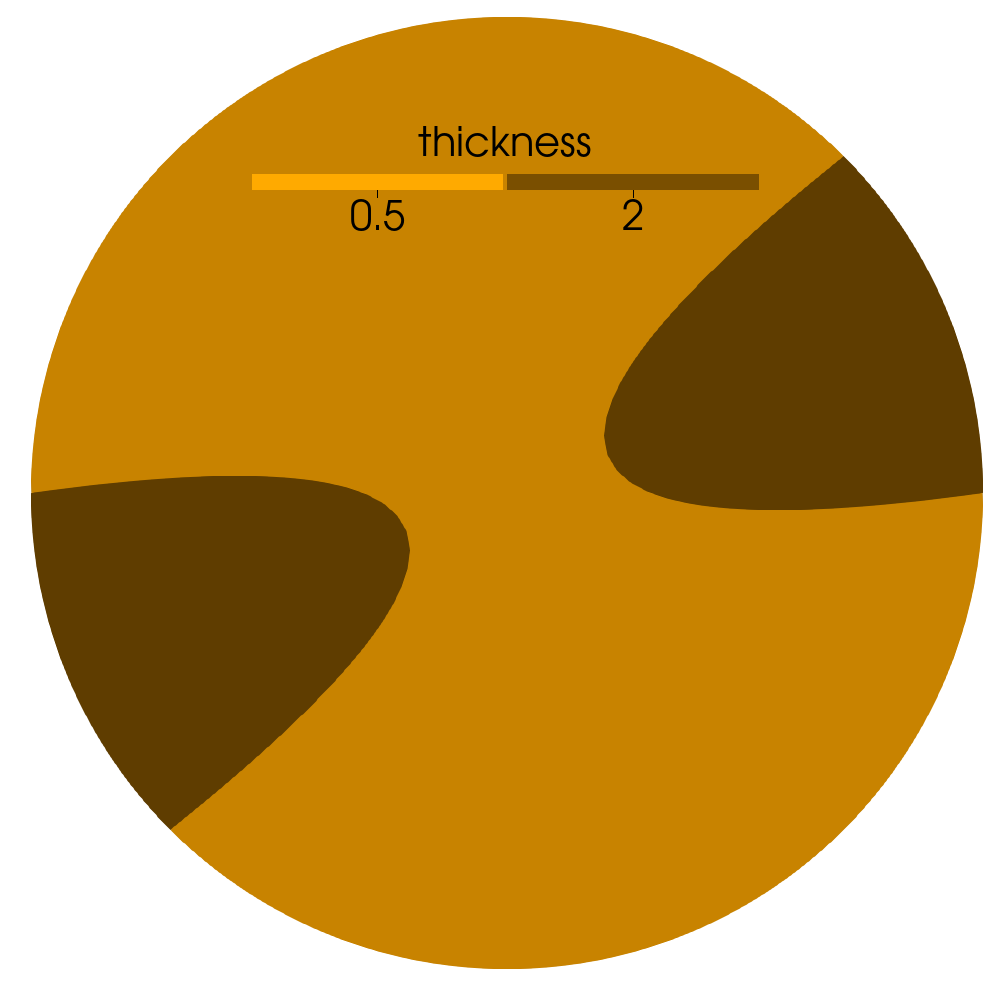
\includegraphics[width=0.25\linewidth]{img/het_circle.png}
    \caption{Гетерогенное поле толщин элементов $T$ круглой мембраны.}
    \label{fig:membrane_thickness}
  \end{figure}
  % \begin{wrapfigure}{r}{0.35\textwidth}
  %   \centering
  %   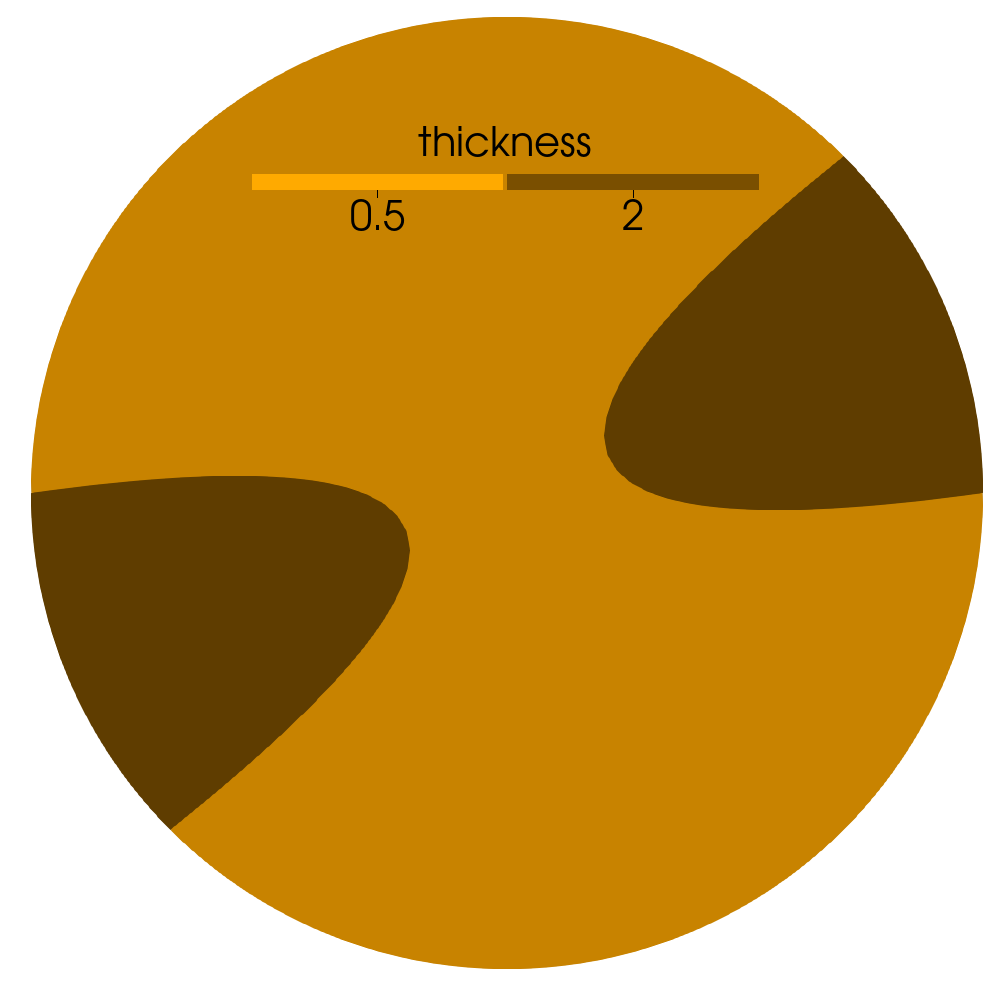
\includegraphics[width=\linewidth]{img/het_circle.png}
  %   \caption{Гетерогенное поле толщин элементов $T$ круглой мембраны.}
  %   \label{fig:membrane_thickness}
  % \end{wrapfigure}
  % Для геометрии с гетерогенным полем толщин референсные значения сдвиговой компоненты поля 2 тензора напряжений Пиолы-Кирхгофа 
  % $\vect S$ (Рисунок \ref{fig:numerical_experiment}) .

  \begin{figure}[H]
    \centering
    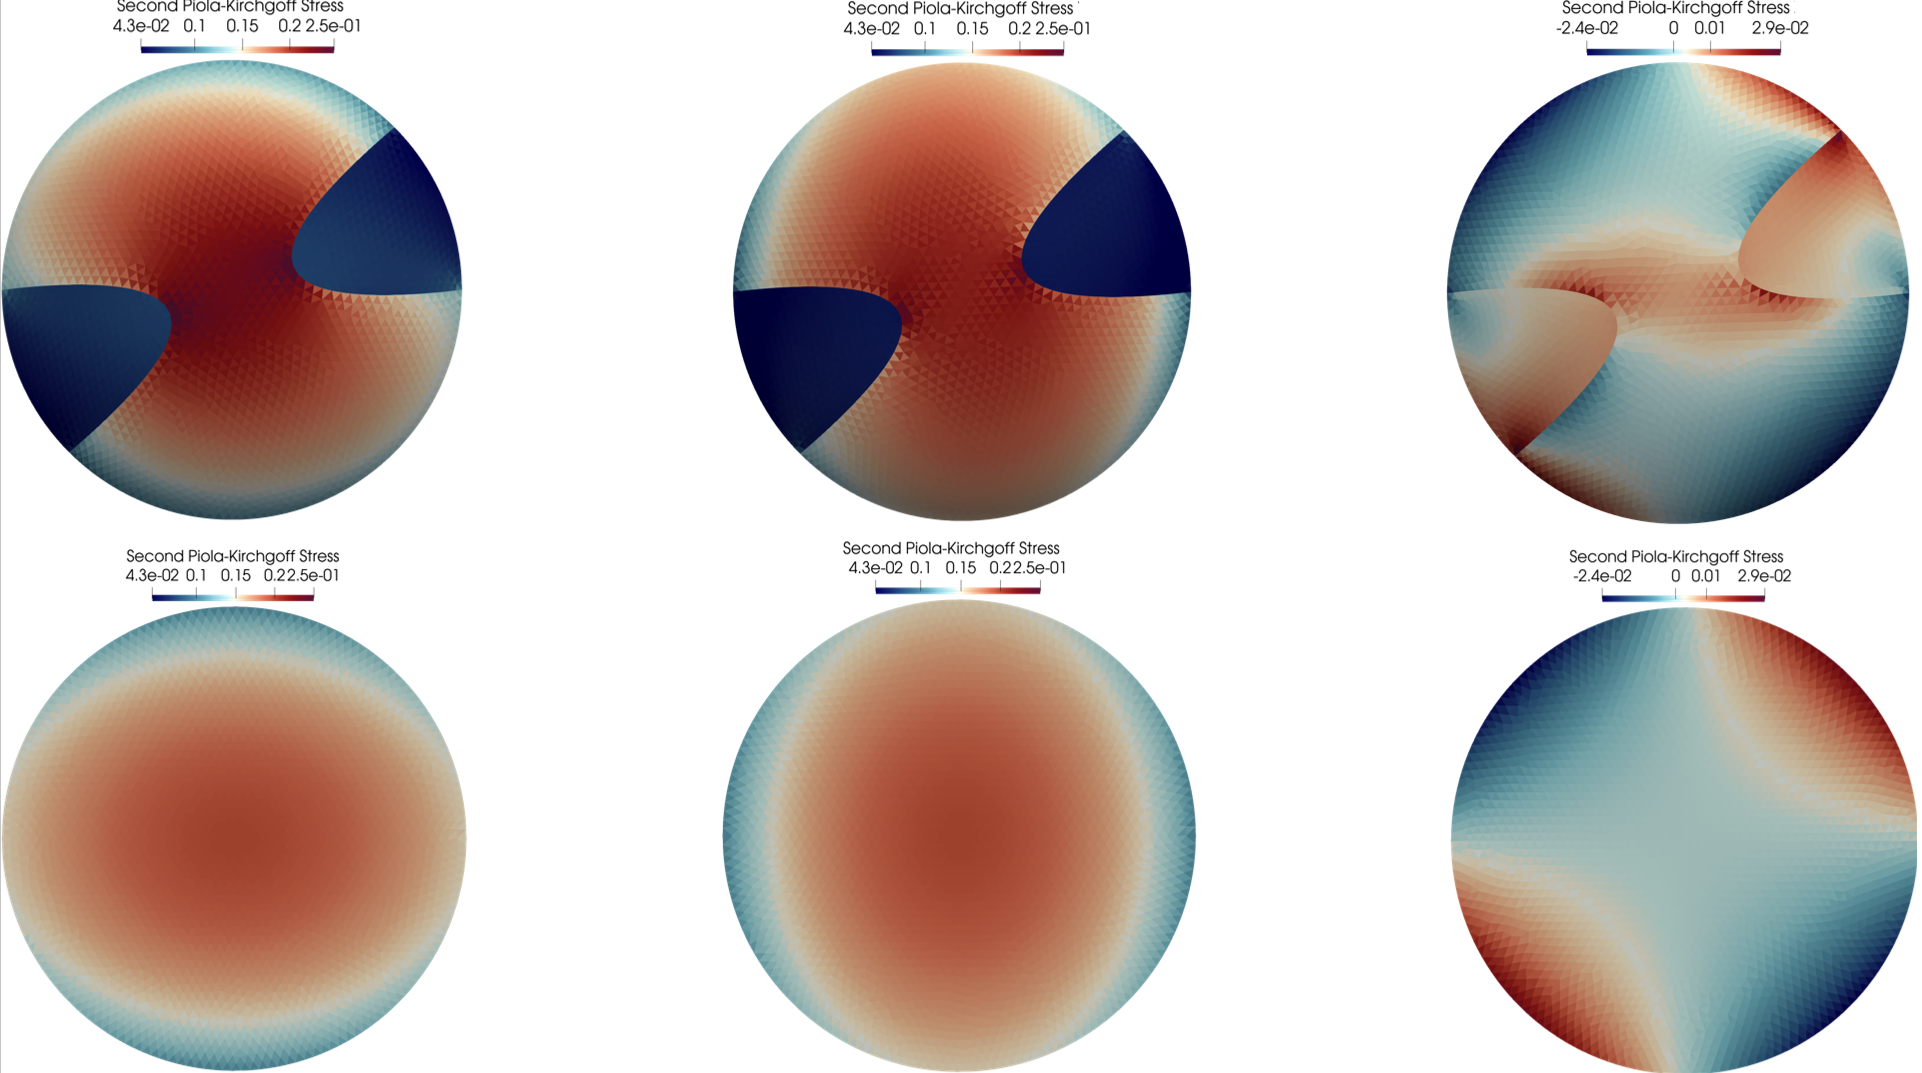
\includegraphics[width=0.7\textwidth]{img/Numerical/ref_stress.png}
    \caption{Поле напряжений $\vect S$ круглой мембраны (пример результата численного эксперимента).}
    \label{fig:numerical_experiment}
  \end{figure}
  
  В результате численного эксперимента на раздутие мембраны с гиперупругим определяющим соотношением CLaNN,
  используя набор данных $D (\{1..10\}, w=\text{1-элемент})$ для обучения, мы получили поле напряжений 2 тензора Пиолы-Кирхгофа 
  $\vect S$ для гомогенной и гетерогенной мембраны по толщине и сравнили его
  с референсными значениями (Рисунок \ref{fig:numerical_experiment}) и построили поле ошибок $\epsilon$ и $\epsilon_{P1}$ (Рисунок \ref{fig:numerical_errors}).
  Сдвиговая компонента напряжений $\vect S_{xy}$ показывает наибольшую ошибку для гетерогенной мембраны, 
  что может быть связано с тем, что данные для сдвиговых компонент не достаточно большие. Поэтому мы последовательно 
  расширяли набор данных для обучения до $D (\{1..10\}, w=\text{5x5})$, $D (\{1..10\}, w=\text{10x10})$, $D (\{1..10\}, w=\text{все поле})$, 
  и построили зависимость интегральной ошибки $\|e\|_{L^2}$ (Формула \ref{eq:l2_abs_stress_cell}) и $\|e\|_{L^2,\,\mathrm{rel}}$ (Формула \ref{eq:l2_rel_stress}) 
  поля напряжения $\vect S$ от размера окна наблюдения $w$ (Рисунок \ref{fig:integral_errors}). 
  В итоге абсолютная интегральная ошибка $\|e\|_{L^2}$  для гетерогенной мембраны уменьшается с увеличением размера окна наблюдения $w$, 
  это может быть связано с тем, что при увеличении размера окна наблюдения мы учитываем больше данных для обучения, в том числе данных 
  для сдвиговых компонент напряжений, например, при отборе ячеек из области ближе к углам квадрата, в который вписана мембрана, 
  сдвиговые компоненты напряжений в этой области вырастают на 1-2 порядка.
  
  
  \begin{figure}[H]
    \centering
    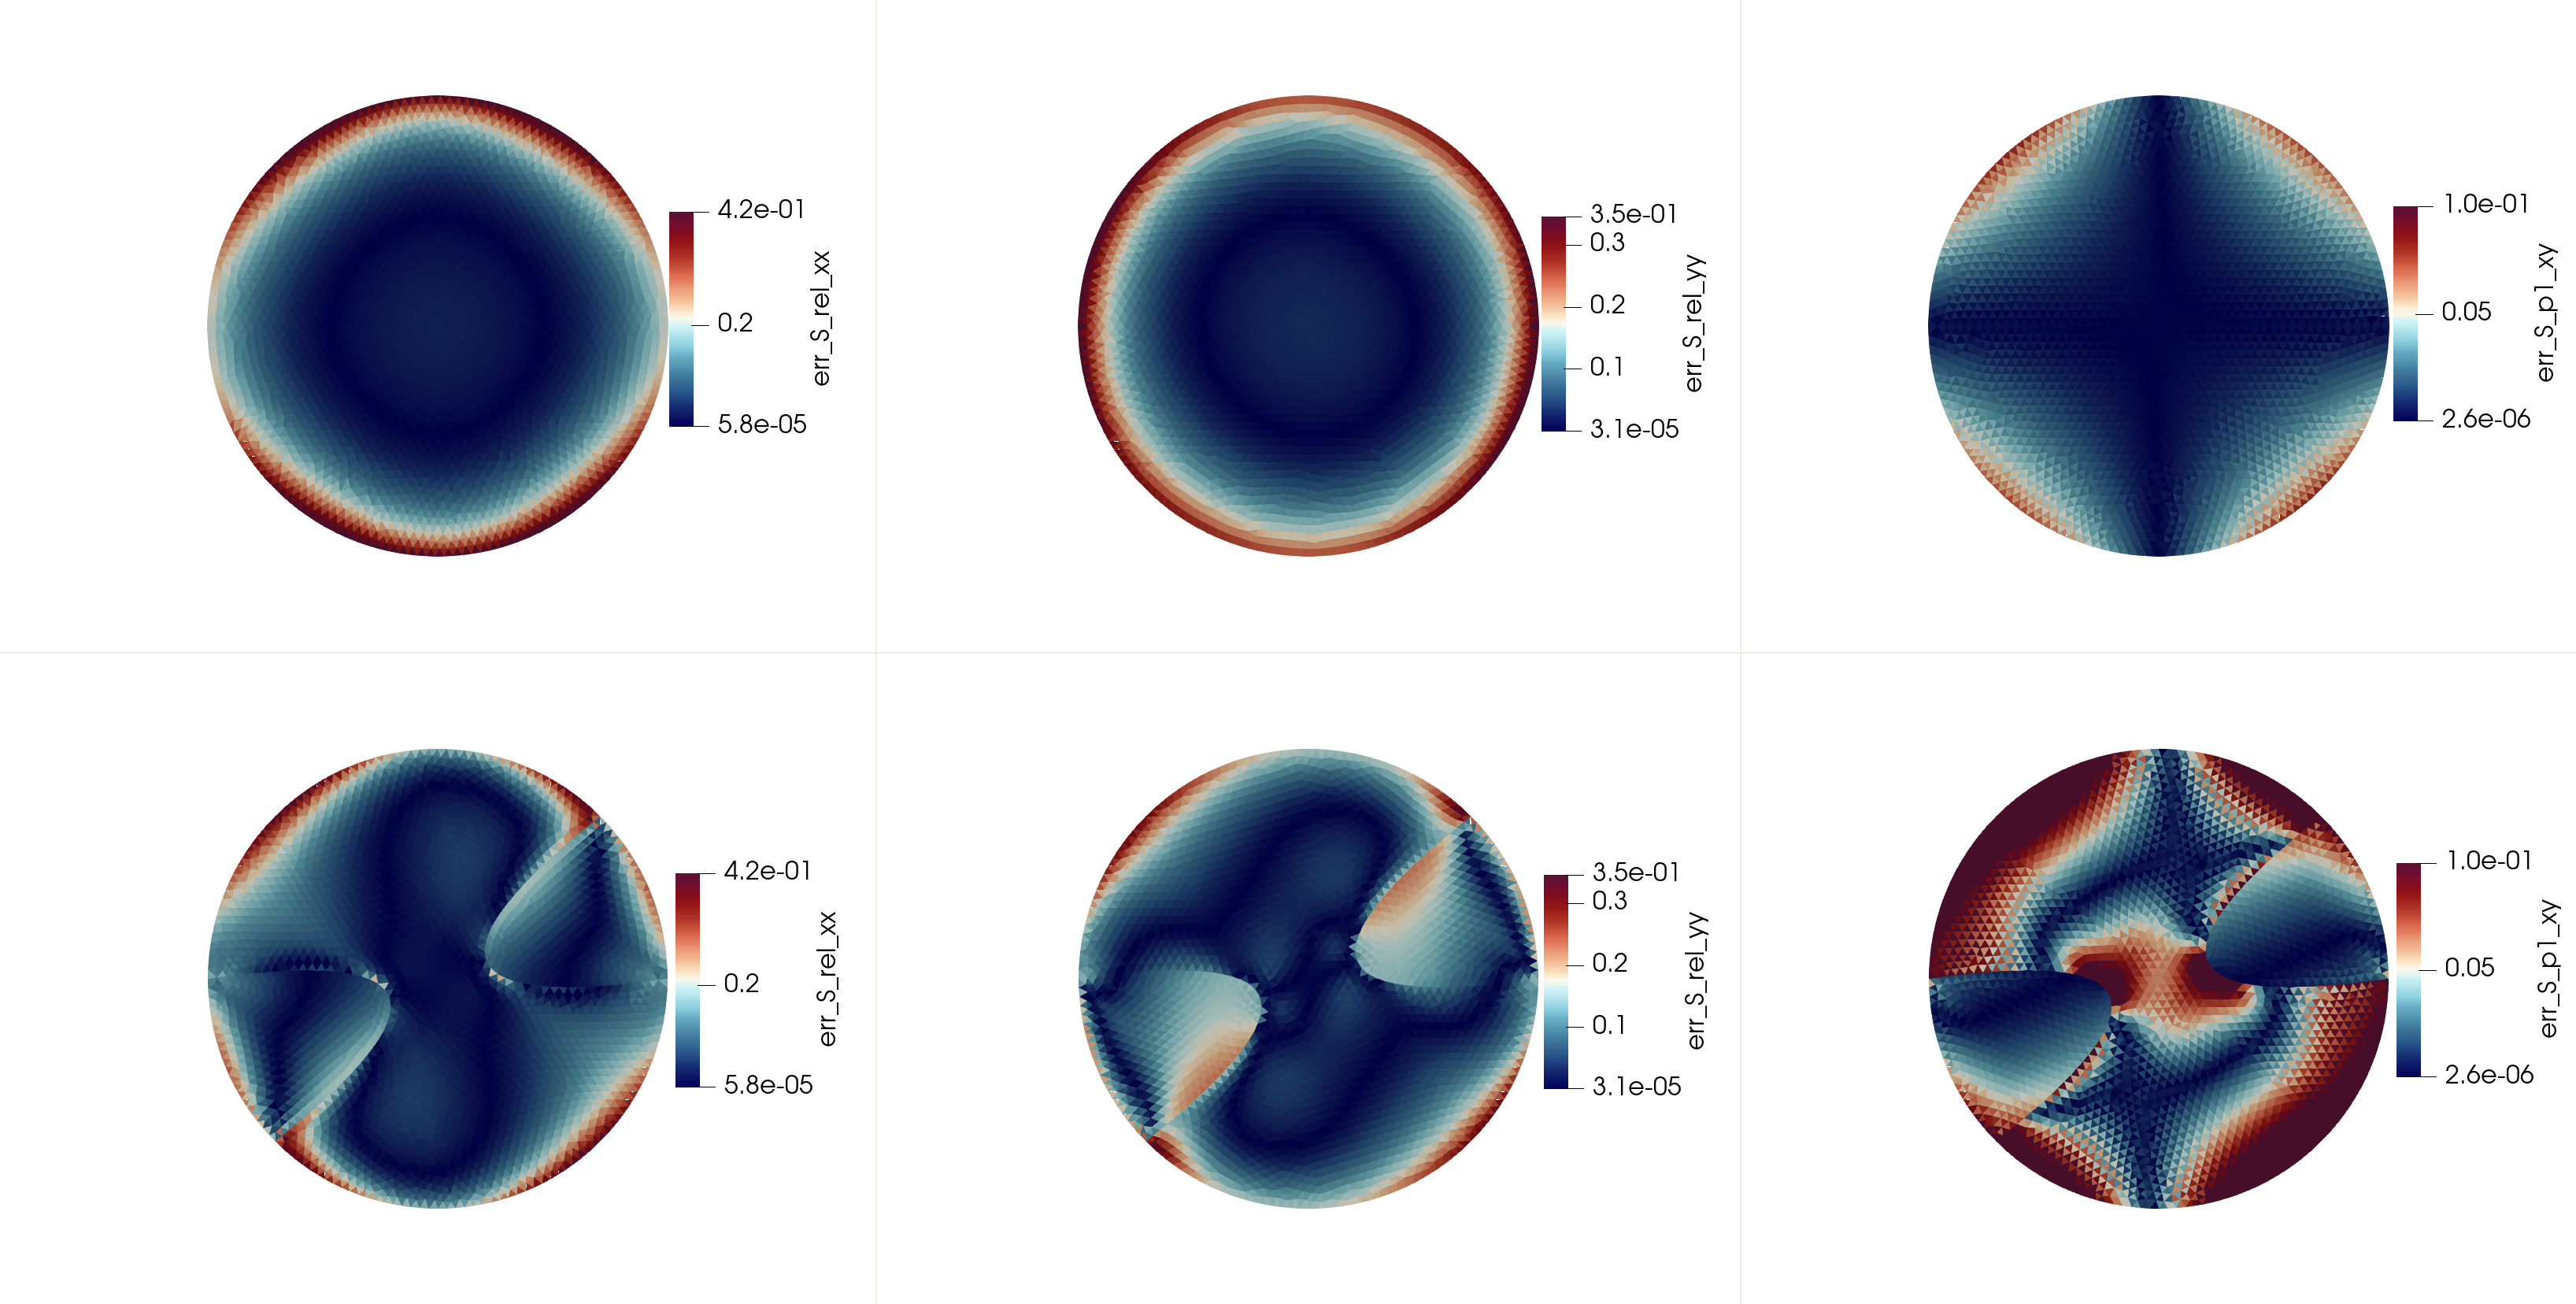
\includegraphics[width=1.0\textwidth]{img/Numerical/errs.png}
    \caption{Поле ошибок между предсказанными и эталонными значениями напряжений.}
    \label{fig:numerical_errors}
  \end{figure}

  \begin{figure}[H]
    \centering
    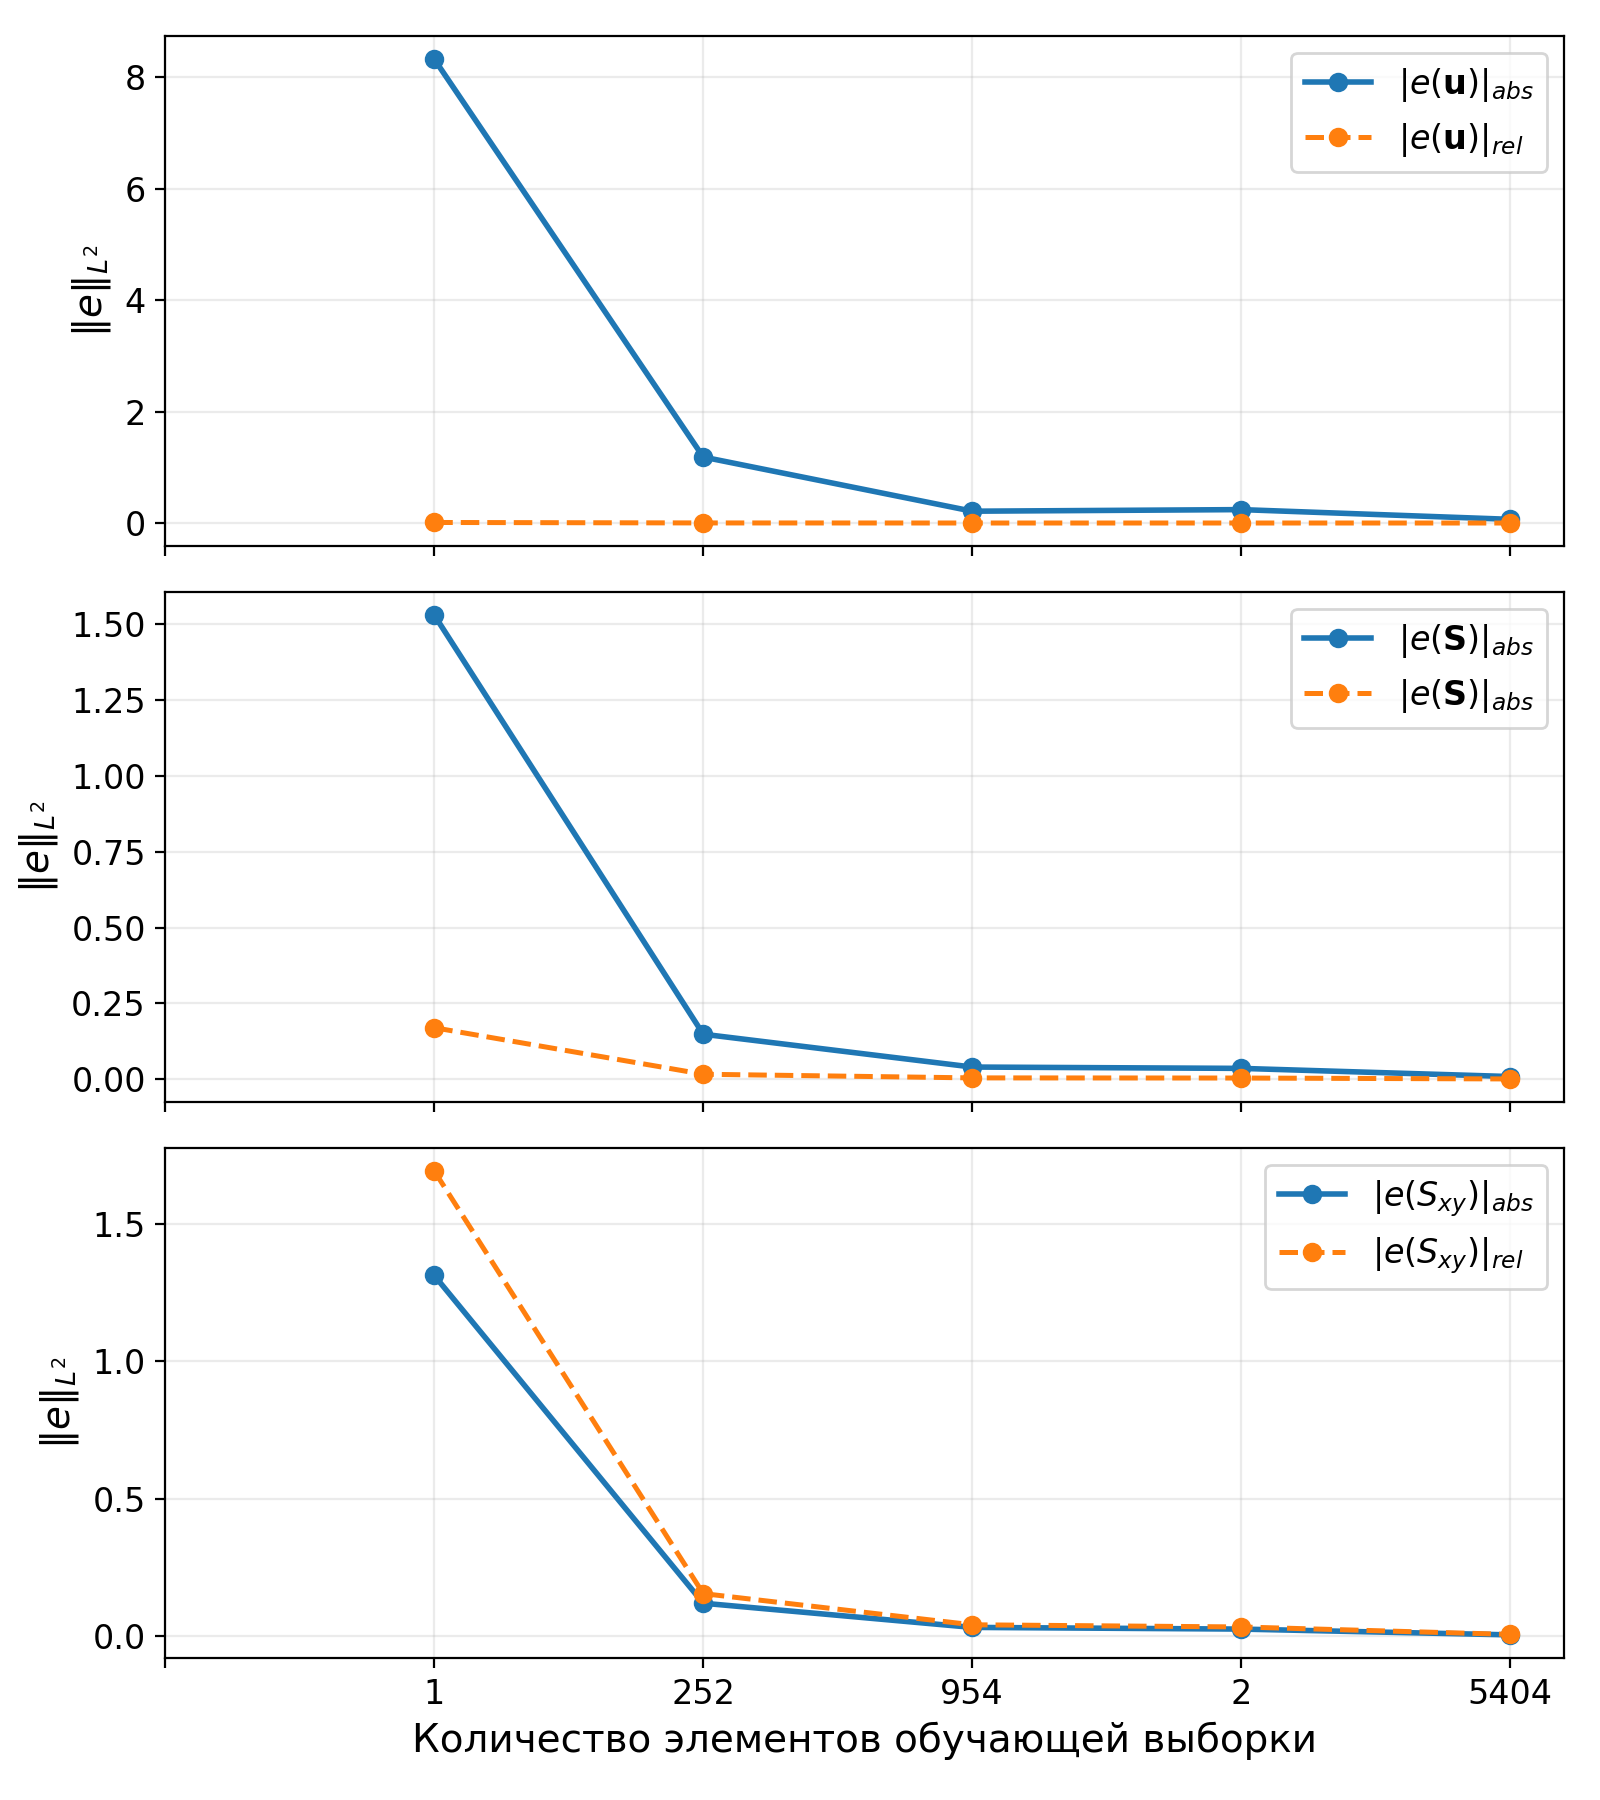
\includegraphics[width=0.5\textwidth]{img/integral_errors.png}
    \caption{Зависимость интегральной ошибки $\|e\|_{L^2}$ и $\|e\|_{L^2,\,\mathrm{rel}}$ от количества элеметов в окне наблюдения размера $w$.}
    \label{fig:integral_errors}
  \end{figure}
  
  % \begin{figure}[H]
  %   \centering
  %   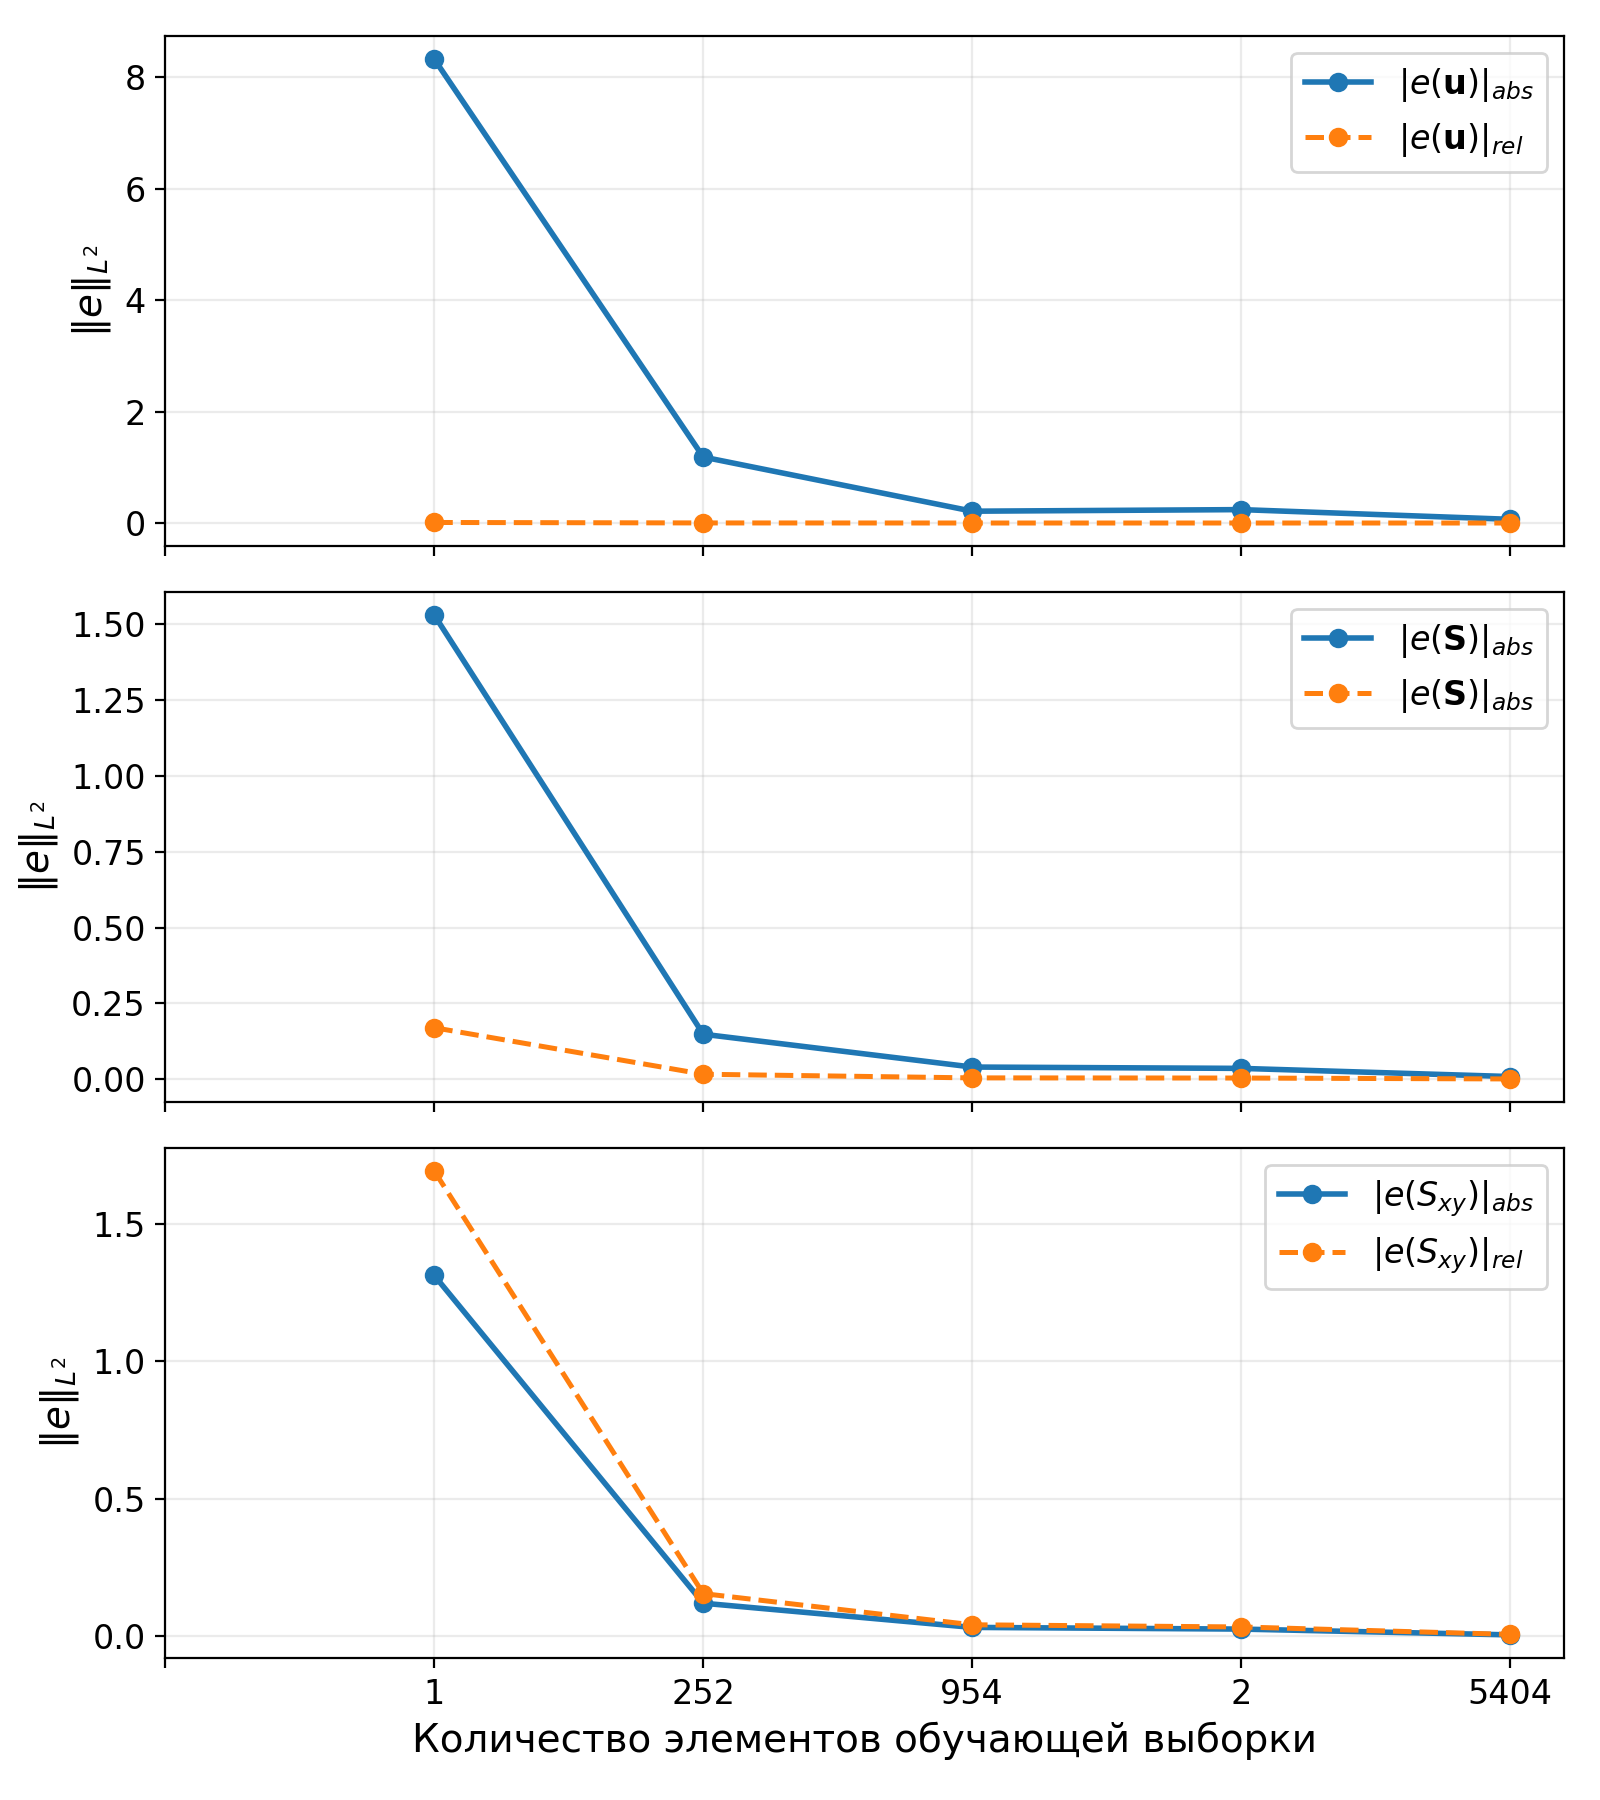
\includegraphics[width=0.7\textwidth]{img/integral_errors.png}
  %   \caption{Интегральные ошибки в зависимости от окна наблюдения.}
  %   \label{fig:_integral_numerical_errors}
  % \end{figure}
  
\subsection{Сравнение вычислительной эффективности CLaNN}

  Благодаря \emph{выпуклости} потенциальной энергии деформации $\psi(\boldsymbol\xi)$ в CLaNN задача стационарного равновесия формулируется
  как гладкая выпуклая минимизация. Это позволяет использовать градиентные и второпорядковые методы со строгими гарантиями сходимости
  (квазиньютон, Ньютона и тд)
  и предсказуемой сложностью до заданной точности \cite{BoydVandenberghe2004,Nesterov2004,NocedalWright2006,ConnGouldToint2000}.
  В окрестности минимума сильная выпуклость и липшицевость гессиана обеспечивают локально квадратичную сходимость Ньютона,
  а квазиньютоновские схемы (L\textendash BFGS) дают сверхлинейные скорости \cite{NocedalWright2006}.

  % \paragraph{Data-drevin модели без выпуклости.}
  В таблично-заданных/локально-интерполяционных DD-моделях (в т.ч.\ k-NN, IDW) выпуклость энергии, как правило, не гарантируется,
  а функция отклика может быть негладкой. Это приводит к невыпуклой постановке с множеством стационарных точек и
  отсутствием глобальных гарантий у классических квазиньютоновских методов. На практике применяются
  квазистатические/релаксационные стратегии: (добавить описание) \cite{KirchdoerferOrtiz2016,KirchdoerferOrtiz2017}.
  Такие методы устойчивы, но, как правило, требуют существенно большего числа шагов нагружения и внутренних итераций
  (а также повторяющихся k-NN/IDW-запросов), что приводит к росту времени расчёта.

  Мы сравнили время решения для CLaNN, классической гиперупругой модели Нео\textendash Гука и DD-модели мембраны, описанной в \cite{xi2023}.
  Задача: раздувание закреплённой круглой мембраны, $R{=}25$ мм, равномерное давление, две конфигурации по толщине $T$ (гомогенная и гетерогенная; см. рис.~\ref{fig:membrane_thickness}).
  Для CLaNN обучаем на наборе данных $D(\{1..10\},\,w{=}\text{1-элемент})$; для сравнения используем DD-модель на основе 
  kNN и IDW, которые работает в пространстве деформаций Лапласа и функций отклика $(\vect{\xi}, \vect{r})$, 
  которые были вычислены из $D(\{1..10\},\,w{=}\text{10}\times\text{10})$ \cite{xi2023}.
  Численное решение выполняем в одной и той же КЭ-постановке для мембранной задачи. 
  Все варианты останавливаем по одинаковым нормам допускам по невязке.

\begin{table}[htbp]
\centering
\caption{Время расчёта (сек) на задаче раздувания: гомогенная vs гетерогенная толщина}
\label{tab:experiments_summary}
\begin{tabular}{|l|c|c|}
\hline
\textbf{Метод} & \textbf{Гомогенная} & \textbf{Гетерогенная} \\
\hline
CLaNN & 512 & 329  \\
\hline
Neo-Hooke & не замерил & не замерил\\
\hline
kNN & 993 & -- \\
\hline
\end{tabular}
\end{table}

  На одинаковой сетке и допусках CLaNN достигает решения сравнимым числом глобальных итераций с Нео\textendash Гуком
  (за счёт выпуклости и корректной кривизны энергии в ICNN), существенно опережая DD-модель по времени расчета
  за счёт отсутствия внешних проекций на данные и дорогих k-NN/IDW-запросов на каждой итерации.
  Также стоит отметить невозможность расчета DD-модели на гетерогенной толщине без линейной интерполяции данных в близи нуля, 
  что может происходить из-за нехватки данных для в этой области деформаций.


